% !TEX root       = ./type_name.tex
% !TEX program    = pdflatex
% !TEX encoding   = utf-8
% !TEX spellcheck = de_DE_frami
%=======================================================================
\chapter{Implementation} \label{ch:implementation}
This chapter will discuss about the procedures involved such as flashing the router with OpenWrt, building the OpenWrt firmware with OVS modules, configuring OVS, setting up RADIUS server in a virtual machine and creating a MySQL database with custom table for access to out port id etc.
\section{Building and Flashing Custom OpenWrt Firmware}
To build the custom firmware for the OpenWrt, we use the \textit{make menuconfig} command in terminal from the directory where the OpenWrt repository has been cloned. The following steps will explain which modules to choose from the Menu and to compile the custom build.
\begin{enumerate}
	\item Navigate to the directory \textit{<buildroot\_dir>} in terminal and then enter the command \textit{make menuconfig}.
	\item In the menu that appears, select the target system by using the arrows and enter key to navigate the menu.
	\item In the target system, choose \textbf{Atheros AR7xxx/AR9xxx}.
	\item Now, select target profile and choose \textbf{TP-Link WDR4300} from the list.
	\item In the main configuration menu, select the \textbf{Luci} menu and enable luci web interface.
	\item Now, going back to the main menu, choose the Network option in the list.
	\item	Within the Network menu, select the sub menu \textbf{Open Vswitch} as shown in figure\ref{fig:openvswitch} and enable all options using space key <*>.
	\item	In the Network menu, first de-select the option \textbf{Wpad mini} and then select \textbf{Hostapd} as shown in figure\ref{fig:hostapd} with full features. This provides the necessary enterprise 802.1x authentication features.
	\item	In the main configuration menu, navigate to \textbf{Utilities} option and select editors and choose either \textbf{vi} or \textbf{nano} as the text editor of choice.
	\item	Exit the menu and select save to save the configuration.
	\item	Back in the terminal, enter the command \textit{make world}. This will compile the changes made in the configuration and build the firmware for the selected hardware profile, in this case TP-Link WDR4300.
	\item	The freshly built images are available in the root directory of OpenWrt \textit{<buildroot\_dir>/bin/ar71xxx}.
	\item	Connect the router to the computer via ethernet and login to the OEM interface using the ip 192.168.0.1 with user/pass as admin/admin.
	\item	Select the option firmware upgrade in the device settings.
	\item	In the OpenWrt bin directory, select the image \textit{openwrt-ar71xx-generic-tl-wdr4300-v1-squashfs-factory.bin} and rename it to 
	\textit{wdr4300v1\_en\_3\_14\_3\_up\_boot(150518).bin}.
	\item	Now, in the OEM web interface, select the renamed file and choose upgrade. It will update the router and reboot.
	\item	OpenWrt has been successfully installed in the router.
	
\end{enumerate}

  \begin{figure}[H]
 	\centering
 	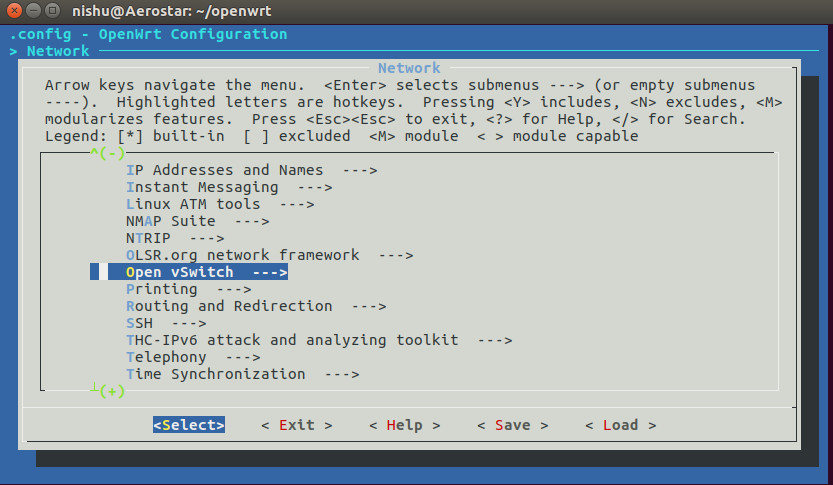
\includegraphics[width=1.0\linewidth]{network-ovs}
 	\caption {Open vSwitch option in OpenWrt build configuration menu}
 	\label{fig:openvswitch}
 	\vspace{-10pt}
 \end{figure}

 \begin{figure}[H]
	\centering
	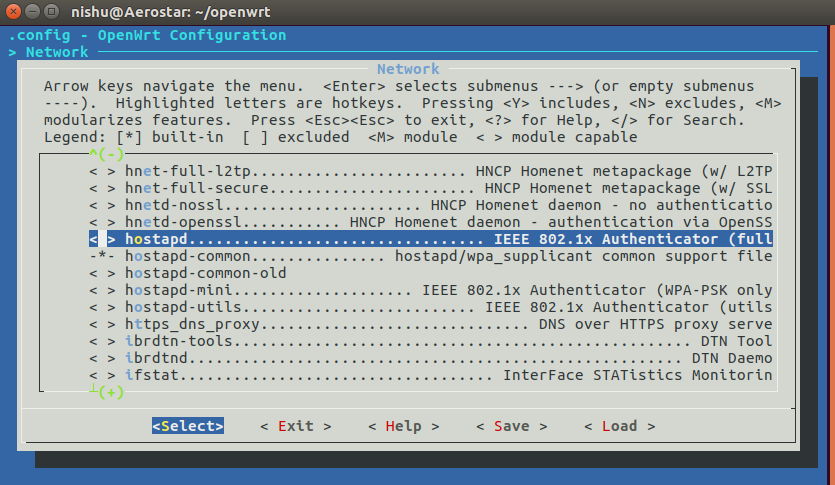
\includegraphics[width=1.0\linewidth]{network-hostapd}
	\caption {Hostapd option in OpenWrt build configuration menu}
	\label{fig:hostapd}
	\vspace{-10pt}
\end{figure}
\section{Router Configuration}
The router has been freshly updated with the OpenWrt firmware. To configure the router, it is first connected via shell which will be discussed below.

The router is first connected via the shell using the command \textit{sudo ssh 192.168.1.1} as seen in the test layout \ref{fig:test-layout}. This will open a OpenWrt configuration terminal that look like in the figure \ref{fig:OpenWrt_terminal}.

The wireless configuration has to be modified to create two ssid's, this can be accessed using the internal editor with the command \textit{nano /etc/config/wireless}. the configuration contains all the information related to the wireless module. In the configuration, there are two device names and only these two needs to be modified. The device configured to use a RADIUS server in the server option and the key, the ssid's are changed to OpenWrt and OpenWrt 5G respectively. The configuration will look like as shown below after modification. The complete configuration can be accessed from the appendix 

\nameref{app:sec:wireless_config}
	\begin{lstlisting}

config wifi-iface
option device 'radio0'
option mode 'ap'
option ssid 'OpenWrt'
option server '192.168.1.169'
option key 'testing123'
option encryption 'wpa2'
option network 'wifi'

config wifi-iface
option device 'radio1'
option mode 'ap'
option server '192.168.1.169'
option key 'testing123'
option ssid 'OpenWrt 5G'
option encryption 'wpa2'
option network 'wifi'
\end{lstlisting}

The second step would be to modify the network configuration in order to create two separate networks with bridge \textit{br-lan} for the interface eth0.1 hosting the network \textit{192.168.1.1} and the bridge \textit{br-wifi} for the interfaces eth0.2, wlan0, wlan1 hosting the second network \textit{192.168.3.1} for which the client is assigned a dhcp post authentication. Separating the rest of the ports as individual interfaces allow them to be configured with OVS bridge which can be seen in the configuration below. The full configuration file is added in the appendix of this document \nameref{app:sec:Network_config}

\begin{lstlisting}
config interface 'lan'
option type 'bridge'
option ifname 'eth0.1'
option proto 'static'
option ipaddr '192.168.1.1'
option netmask '255.255.255.0'
option ip6assign '60'

config interface 'wifi'
option type 'bridge'
option ifname 'eth0.2'
option proto 'static'
option ipaddr '192.168.3.1'
option netmask '255.255.255.0'
option ip6assign '60'

config interface 'lan2'
option ifname 'eth0.2'

config interface 'lan3'
option ifname 'eth0.3'

config interface 'lan4'
option ifname 'eth0.4'

config interface 'lan5'
option ifname 'eth0.5'

\end{lstlisting}

To enable the new network to provide DHCP to the devices that connects to the OVS bridge, the DHCP has to be modified to accomodate the new network. This can be easily access in the editor with the commans \textit{nano /etc/config/dhcp} and the configuration shown below  is added to the file and saved.

\begin{lstlisting}
config dhcp 'lan4'
option interface 'lan4'
option ignore '1'
\end{lstlisting}

Once the configurations are complete, the router is restarted to apply the changes. It is verified by logging into the web interface with the ip \textit{192.168.1.1}. This will open a LuCi web interface in the browser and shows the routers status and reflects the changes that were made with the configuration.

%\begin{enumerate}
%	\item Connect to the router using the command ssh 192.168.1.1 and accept the key signatures. It will now show the configuration window with \textit{root@openwrt}.
%	\item To create two wifi networks in the router, first open the networks configuration in the editor using vi or nano with the following command \textit{nano /ect/config/wireless}.
%	\item The configurations are changed to look like the one shown below.
%	\begin{lstlisting}
%	
%	config wifi-iface
%	option device 'radio0'
%	option mode 'ap'
%	option ssid 'OpenWrt'
%	option server '192.168.1.169'
%	option key 'testing123'
%	option encryption 'wpa2'
%	option network 'wifi'
%	
%	config wifi-iface
%	option device 'radio1'
%	option mode 'ap'
%	option server '192.168.1.169'
%	option key 'testing123'
%	option ssid 'OpenWrt 5G'
%	option encryption 'wpa2'
%	option network 'wifi'
%	\end{lstlisting}
%	\item Save the file using ctrl + x and enter. Now open the network configuration file from the command \textit{nano /etc/config/network} and change it to look as shown below.
%	\begin{lstlisting}
%	config interface 'lan'
%	option type 'bridge'
%	option ifname 'eth0.2'
%	option proto 'static'
%	option ipaddr '192.168.1.1'
%	option netmask '255.255.255.0'
%	option ip6assign '60'
%	
%	config interface 'wifi'
%	option type 'bridge'
%	option ifname 'eth0.3'
%	option proto 'static'
%	option ipaddr '192.168.3.1'
%	option netmask '255.255.255.0'
%	option ip6assign '60'
%	
%	config interface 'lan3'
%	option ifname 'eth0.3'
%	
%	config interface 'lan4'
%	option ifname 'eth0.4'
%	
%	config interface 'lan5'
%	option ifname 'eth0.5'
%	
%	config switch_vlan
%	option device 'switch0'
%	option vlan '2'
%	option ports '2 0t'
%	option ipaddr '192.168.3.1'
%	option netmask '255.255.255.0'
%	option ip6assign '60'
%
%	\end{lstlisting}
%	\item The DHCP for the second network is configured in the file \textit{/etc/config/dhcp} and the following entry is added to the file.
%	\begin{lstlisting}
%	config dhcp 'lan4'
%		option interface 'lan4'
%		option ignore '1'
%	\end{lstlisting}
%	\item Save the configuration and reboot the router.
%	\item The web interface of OpenWrt can be opened using the ip \textbf{192.168.1.1}. Enable the wireless interfaces in the Networks menu as they are disabled by default. Now, there should be two network ssid openwrt and openwrt 5G available in the client device.
%	
%\end{enumerate}
  \begin{figure}[H]
	\centering
	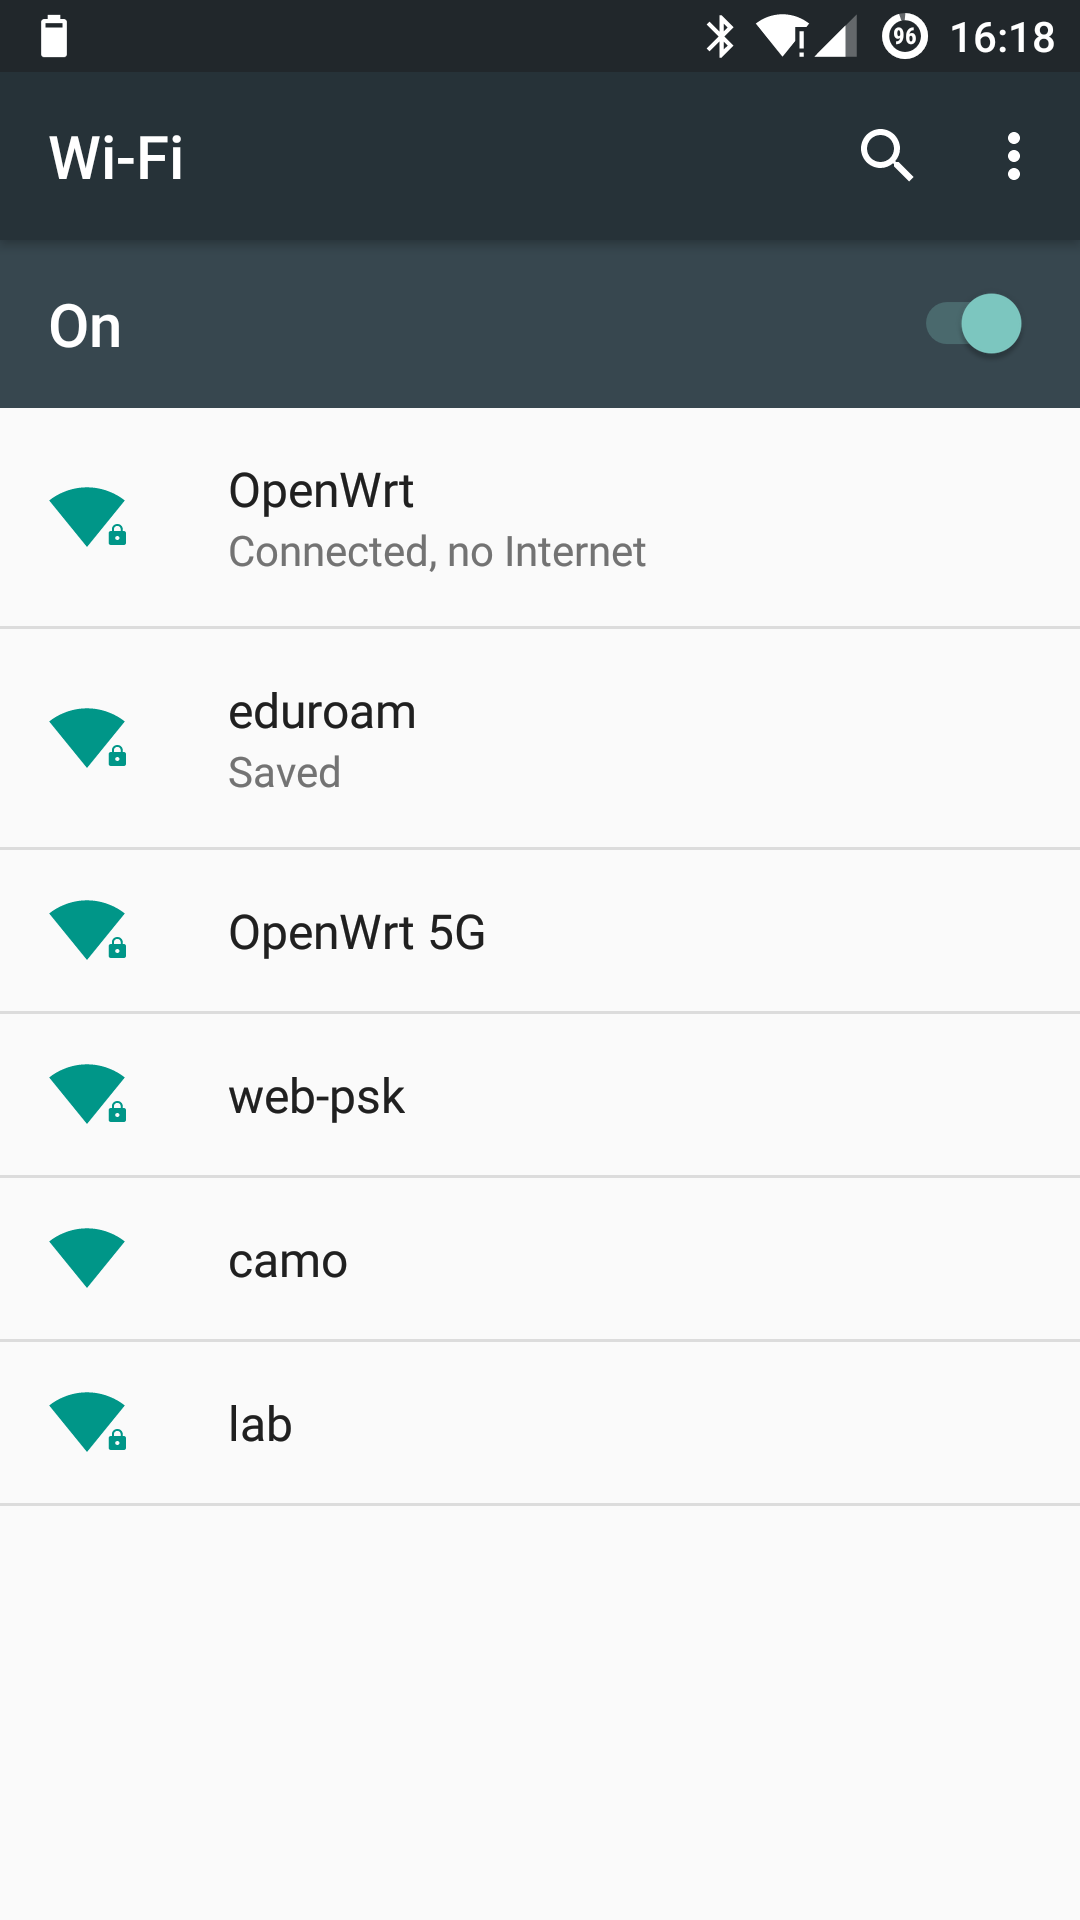
\includegraphics[width=10cm, height=13cm,keepaspectratio]{two-ssid}
	\caption {SSID's OpenWrt and OpenWrt 5G Available on client device}
	\label{fig:two-ssid}
	\vspace{-10pt}
\end{figure}
\section{Configuring Open vSwitch}
The Open vSwitch is configured to connect with the RYU controller and assign ports to be managed by the controller. The configuration is made by using the following commands in the OpenWrt shell terminal.
\begin{enumerate}
	\item Login to OpenWrt router using shell via the command \textit{sudo ssh 192.168.1.1}.
	\item The installation of OVS is checked using the following command \textit{ovs-vsctl show}, if it says there is no such command, then there is no OVS installed. Instead if it shows an empty entry then OVS is installed but not configured.
	\item The OVS bridge is created using the command \textit{ovs-vsctl add-br br0}
	\item To set the controller for OVS, the command \textit{ovs-vsctl set-controller br0 tcp:192.168.1.207:6633} is used, where 6633 is the standard OpenFlow port.
	\item The failsafe mode in a OVS switch tell the switch how to function in case of a connection failure with the controller. There are two modes, \textbf{secure} and \textbf{stand\_alone}. The \textbf{secure} mode will not allow any packets to pass through whereas the \textbf{stand\_alone} mode will function as a normal switch. For this project, the failsafe mode is set to secure to isolate the network using the following command \textit{ovs-vsctl set-fail-mode br0 secure}.
	\item The ports that needs to be managed are added to the bridge using the commands
	\begin{lstlisting}
		ovs-vsctl add-port br0 eth0.3
		ovs-vsctl add-port br0 eth0.4
		ovs-vsctl add-port br0 eth0.5
	\end{lstlisting}
	\item The configuration is verified by the command ovs-vsctl show, this will show the configuration that was made in the OVS.
	
\end{enumerate}
\section{MySQL Setup}
The following steps explain the procedure to install and configure MySQL server and populate its database to work with Freeradius server on the ubuntu virtual machine.
\begin{enumerate}
	\item MySQL is downloaded and installed on the Linux PC using the following command in terminal \textit{sudo apt-get install mysql-server}
	\item Once the server is installed, a database called radius is created using the following command. 
	\begin{lstlisting}
	mysql -uroot -p
	CREATE DATABASE radius;
		GRANT ALL ON radius.* TO radius@localhost IDENTIFIED BY "radpass";
	exit
	\end{lstlisting}
	
	\item The schema for \textbf{Freeradius} is added to the database using the following command: \textit{mysql -u root -p radius < /etc/freeradius/sql/mysql/schema.sql}
	\item	To manage the database a\textbf{ PHPMyadmin} tool is installed and configured to connect with the MySQL database. It provides a web interface to manipulate the complete database.
	\item	\textbf{Radcheck} table contains the user credentials, it was modified to add a port id column where a port id is manually assigned to each user.
	
\end{enumerate}
\section{Installing Ubuntu Virtual Machine and Freeradius Server \cite{Freeradius_install}}
The initial method to configure the Freeradius and MySQL server within the OpenWrt router failed due to memory restrictions. Therefore, the Freeradius is installed in an Ubuntu virtual machine configured in a Virtual Box environment. The steps involved is discussed as follows.
\begin{enumerate}
	\item A new virtual machine is created using the latest \textit{Ubuntu 16.10 iso} image in Virtual Box with 2GB RAM and the network is bridged with eth1 which is connected to the internet, initially to download and install Freeradius.
	\item Freeradius is downloaded and installed using the following command \textit{sudo apt-get install freeradius}.
	\item The radius service is started using the command \textit{freeradius -x} if it throws an error, then error shown is debugged and fixed.
	\item Edit the \textbf{clients.config} file in \textit{/etc/freeradius/} directory and add the following line in the file 
	\begin{lstlisting}
	client 192.168.1.1{
			secret = testing123
	}
	\end{lstlisting}
	
	\item Now, the Freeradius server is configured to use MySQL database for authentication and accounting. To configure, the file \textbf{radiusd.conf} in the directory \textit{/etc/freeradius/} and the following steps are taken.
	\begin{enumerate}
		\item Include \textbf{sql.conf} is uncommented.
		\item In the file \textbf{sql.conf} which is in the same directory, the database name is added in the line \textit{database = “mysql”}
		\item Under connection info add 
		\begin{lstlisting}
		server = "localhost"
		login = "radius"
		password = "radpass"
		radius_db = "radius"
		\end{lstlisting}
	\end{enumerate}
	
	\item To store the clients MAC address in the DB, the calling-station-id information is added in the schema file \textbf{dialup.conf} which resides in \textit{/etc/freeradius/sql/mysql/} directory. The information is added in the \textbf{radpostauth} table under Authentication Logging Queries section in the file.
	\begin{lstlisting}
	postauth_query = "REPLACE INTO ${postauth_table} \
	(user, pass, reply, date, CallingStationId) \
	VALUES ( \
	'%{User-Name}', \
	'%{%{User-Password}:-%{Chap-Password}}', \
	'%{reply:Packet-Type}', '%S', '%{Calling-Station-Id}')"
	\end{lstlisting}

	\item Finally, the Freeradius server is tested using the following to check if authentication works properly by using the following command \textit{radtest test radpass 127.0.0.1 0 testing123} where testing123 is the radius key configured in the access point. Access-accept message is received when authentication is successful else, the error can be debugged using the command \textit{sudo freeradius -X} in the terminal
	
\end{enumerate}
